\documentclass{tmr}
\usepackage[utf8x]{inputenc}
%\usepackage[T1]{fontenc}

\usepackage{url}

\newcommand\degree{º}
\newcommand\Cpp{C\kern-.05em\raise.45ex\hbox{\tiny{++}}}
\title{A Haskell sound specification DSL: Ludic support and deep immersion in Nordic technology-supported LARP}
\author{Henrik Bäärnhielm\email{redstar@kth.se}}
\author{Daniel Sundström\email{daniel@monkeydancers.com}}
\author{Mikael Vejdemo-Johansson\email{mikael@johanssons.org}}

\begin{document}

\begin{introduction}
  In March 2013, the battleship Småland in the Gothenburg harbor was
  transformed into a spaceship, the Monitor Celestra of the
  Battlestar Galactica fleet, for a three day Live Action Roleplaying
  Game. To support the feeling of total immersion into the game world,
  we built extensive technological support for the game experience,
  including a sound system with a programmable control layer written
  in Haskell. 

  In this article we will describe this control layer and our
  experiences building and using it for this game project.
\end{introduction}


\emph{The Monitor Celestra} is a game that transformed a World War II era battleship into a space ship, inviting the participants of the game to enter the Battlestar Galactica~\cite{larson_battlestar_1978} universe and forge their own path into the future. The game, a Nordic Style Live Action Roleplaying Game (LARP) assigns roles to the participants -- as crew, passengers and refugees on board the space ship -- and act out the resulting story within a framework of plots, story lines and clues. The medium differs from theatre plays in the lack of a script and from improvised theatre in the lack of an audience -- to consume the medium is to participate in it.

Nordic Style LARPs are characterized, among other things, by a strong focus on immersion. The goal is for participants to feel embedded in the game world without the distraction of the real world disturbing the fiction. In recent years, more and more games have been organized that include technological support to improve the feeling of immersion into the game world.

For \emph{The Monitor Celestra}, full immersion was implemented using a number of different techniques: the signage of the ship was replaced with signs that were
in the Battlestar Galactica aesthetic, the ship
had custom-built control panels controlled a space dynamics simulator, and the game
master team had the ability to trigger a large array of scripted, partially scripted or improvised events that launch sounds and influence the ship control panels to convey the story.

An important part of this immersion was 15 pairs of
loudspeakers, each pair hooked up to a Raspberry Pi~\cite{rpi} and
connected to a wired ethernet network. These loudspeakers played
localized sound effects as well as an ambient sound backdrop through
the entire game, drowning out the sounds of inner city Gothenburg and
supporting the game experience by confirming consequences of player
actions through mediated responses.

\section{Background}
\label{sec:background}

LARP is a form of game where participants receive roles and then proceed to enact their roles within a framework of plots, story lines and clues. Traditionally, LARPs have been focused on telling stories in a fantasy/medieval setting, but the form has seen a wider spread of genres over years. LARP has developed into various design schools and style -- mostly based on geographical distribution. Thus, there are Nordic LARPs, American LARPs and Russian LARPs, to name a few~\cite{kp2011}. Each school of design has its own theories on what constitutes a good LARP and what goals one must strive to achieve with the game design, participation and outcome of the game.

In the same tradition as table-top role playing games and improvisation theatre, LARP is played out by players in real time in the same general physical area. Players wear costumes and make props to better simulate their respective characters. In general, participants receive instructions beforehand regarding specific game rules, other characters, shared background information, etc. Organizers define social mechanics and hard game rules for resolving combat, conflicts or sex. 

\subsection{Nordic LARP}

\emph{The Monitor Celestra} belonged to the Nordic LARP school of design. This school could be argued to emphasize a few different points as being major when creating or participating in the experience: 

\begin{itemize}
    \item The game should represent the world as faithfully and completely as possible (games which fulfill this criterion are commonly referred to as $360^{\circ}$ games.) Everything players see and/or experience represents itself within the game -- a gun is a gun, a knife is a knife.
\item Participants should put emotional engagement and experience above achieving in-game goals. Powerful emotional impacts should take precedence when deciding how to move the game forward.
\item The players should control the outcome of the game. While parts of the game might be scripted, the main outcome of the game should be left to the players as far as possible.
\end{itemize}

Due to the nature of the Nordic school of design, games designed within that school tend to focus on moral choices and complex social interactions rather than traditional fantasy stories. There have been games depicting everything from Danish hobos on the road (\emph{The White Road}~\cite{pedersen2008}) and students investigating possessed ladies (\emph{Prosopopeia}~\cite{jonsson2006prosopopeia, montola2006prosopopeia}), to 1950s families hiding from nuclear war (\emph{Ground Zero}~\cite{nordiclarp}) and terminal cancer patients (\emph{Luminescence}~\cite{nordiclarp}).

\subsection{LARP vs. Similar activities}

What separates LARP from other similar activities such as tabletop
roleplaying games, computer games and improvised theatre is still an
open question. Researchers~\cite{montola2012,turku3,henriksen2004}
have pointed to a few main points; 

\begin{itemize}
\item Emotional engagements increased radically when players are physically engaged in the activity~\cite{turku3}.
\item Moral choices and consequences from player actions have larger impact when acted out by other physical players~\cite{turku3}.
\item Players allow themselves more freedom when acting within a ludic circle,\musthavefootnote{\textit{ludic circle}: a shared space of playfulness, from \textit{ludic}: playful} thus allowing for a wider range of emotions, experiences and shared actions~\cite{montola2012,stenros2012}.
\item Reflections on the complexity of social and/or humanistic behavior or models yield a higher level of understanding~\cite{henriksen2004}. Research has shown that when trying to understand complex models of human behaviour, both in extreme situations such as emergencies and in everyday contexts - LARP tend to work very well as tool for exploring motivations, social roles and social systems based on incitements
\end{itemize}

It has been humorously suggested that LARPing may be seen as the ``extreme'' sport of interactive experiences due to the efforts involved with staging and participating in games, the impact on participants and the cumulative effects of player actions and organizer design.

\subsection{Similar Events}

There have been other efforts to use technology to enhance LARP experiences within the game\musthavefootnote{As apart from using techonology for support functions, such as economy, participant management etc.} as a key part of staging the experience, mainly within the Nordic school of LARP design. Historically, these experiments have been conducted by a small number of game designers and writers. Experiences where technology were used in a similar capacity as on \emph{The Monitor Celestra} includes: 

\begin{itemize}
\item \textbf{Prosopopeia: Bardo 1} A technology-enhanced LARP played in the autumn of 2005. Players used technology concealed in an old reel-recorder to communicate with dead spirits.
\item \textbf{Prosopopeia: Momentum} An continuation to the Prosopopeia project, \emph{Momentum} played in the autumn of 2006. Players used a wide variety of technology, including hardware built using custom constructed components to explore and wage battles against forces on the other side of death. 
\item \textbf{Felsäkert Läge} A technology-enhanced LARP in the autumn of 2010 situated in a future, post-apocalyptic world, staged in an abandoned mining town in the north of Sweden. Technology was used to simulated surviving technology from before the catastrophe, telling stories and providing quests, items and treasures for the players to find and use in their own game.
\end{itemize}

An overview of similar experiments (and others) can by found in~\cite{nordiclarp}.

\subsection{Immersive Soundscapes}
Earlier efforts on immersive soundscapes include various implementations in Python, support in most holistic game engines and similar. However, the main difference between these implementations and the system built for \emph{The Monitor Celestra} is the spatial scale. Usually, these soundscapes are meant to be enjoyed by a single person in headphones or a handful of persons in a single or a few rooms. 

The difference in scale between these implementations and the one described in this paper makes comparisons hard to do. Most issues met by the usual implementations were either deemed irrelevant (such as super-focused spatial placement in the scene -- a rough idea was more than enough for a battleship) or too specific (solutions for physical placing loudspeakers in a square room). 

\begin{figure}[H]
  \centering
  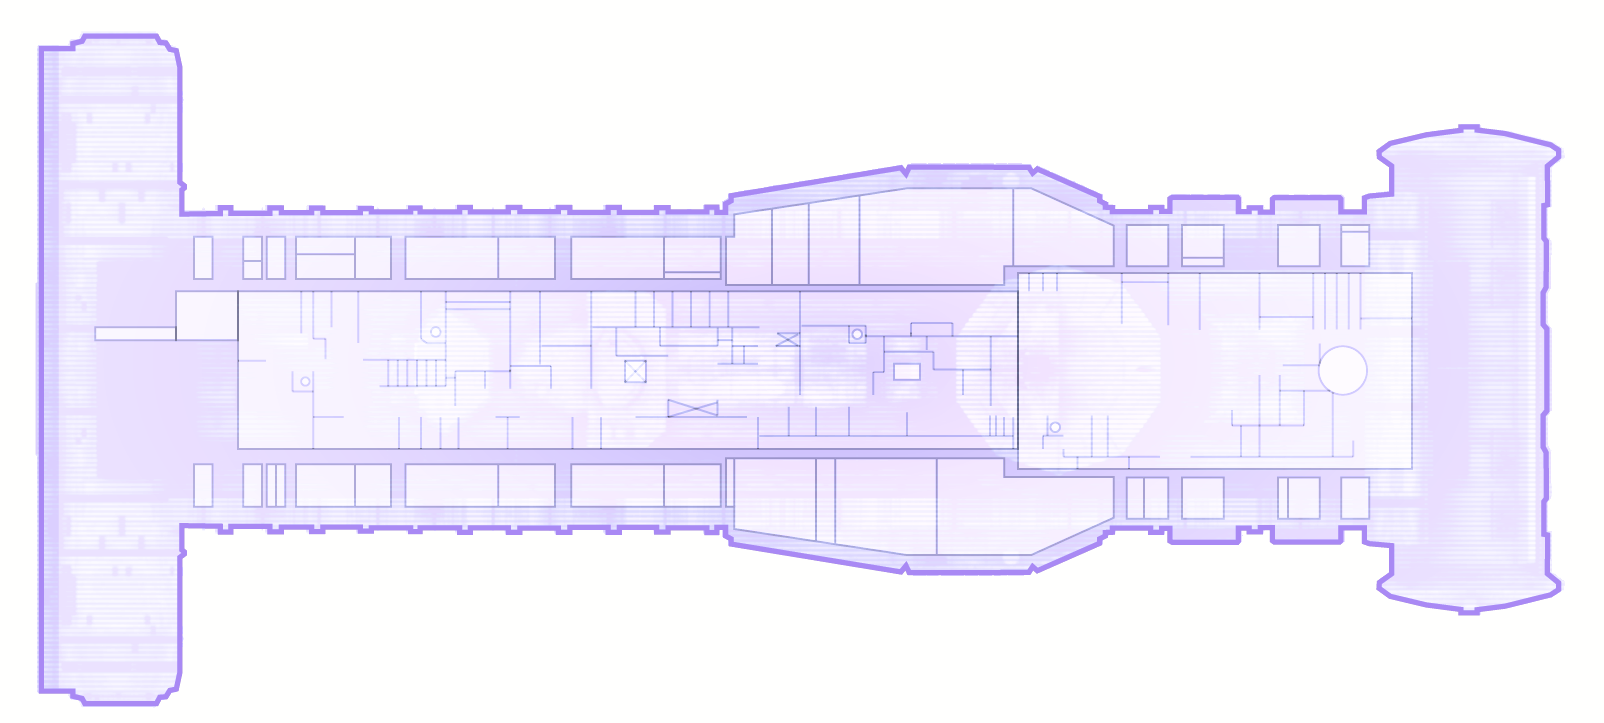
\includegraphics[width=0.6\textwidth]{img/ship}
  \caption{Floor plan of The Monitor Celestra}
  \label{fig:celestra}
\end{figure}

\subsection{Structure of The Monitor Celestra}
Every LARP differs in structure and design according to the design goals, creators and aims with the project. The Monitor Celestra had three runs with 150 participants each, split over three weekends. The runs were separated from each other and played out the same story with different participants (even though some participants bought tickets for all the runs). 

Every run was split into four game sessions of 4--6 hours, with breaks between for sleep and briefings. Food was distributed and eaten while in play. Even though the battleship Småland was equipped with bunks for its crew, fire regulations prohibited sleeping on board the ship. Hence, the participants slept at a nearby hostel between game days.

The story design started out in the setting of Battlestar Galactica: a fleet of refugee spaceships carrying most of the remainder of humanity flee from robot aggressors. In the game, The Celestra is separated from the remaining fleet by accident, and the players have to decide on their actions, while facing various threats: robots hunting them down, colonies with radical political views and demands, and internal conflicts on board the ship. Each of the games ended in a different way, ranging from a valiant effort to save the human race by nuclear suicide taking out a threat before it could reach the rest of the fleet to setting course for deep space and forging a new path for the isolated ship.



%%% Local Variables: 
%%% mode: latex
%%% TeX-engine: default
%%% TeX-master: "tmr"
%%% End: 



\section{Game control system design}
\label{sec:game-control-system}

The technology team for \emph{The Monitor Celestra} settled at a
relatively early stage on an overall design for the game support
technology; the choices made included: \EZY{Work harder to have parallel construction in this bulleted list. It might be easier if you use complete sentences.}
\begin{itemize}
\item Wired ethernet communication for everything, split into three
  different parallel networks: sound, game system, and player hackable. Due to the nature of the 
  play area, parallel network backbones were installed for maximum durability and error management.
\item Communication between game components over \texttt{AMQP} from a RabbitMQ running on a local
game server on the main network. Game logic, world engine and game rules were written in Ruby.
\item Game consoles and GUIs written in HTML5 Canvas rendered on Chromium running in fullscreen.
\item All game consoles must be able to used interchangeably with custom hardware components being plug-and-play.
\item No authentication required within the game network. All published messages can be trusted on a system level. 
\item A single game component responsible for game world, time progression and synchronization; in this case, a rack server running latest stable Ubuntu LTS\@.
\item Connection to external network and Internet through a single point-of-entry, the main game server.
\end{itemize}

The choices were made based on experiences from earlier projects staged
in similar contexts; not-for-profit with volunteers, widest match against available skillsets, relatively uncontrolled environments
and subjected to the wear-and-tear of playing adults. \EZY{This sentence is really awkward}


\section{Sound system design}
\label{sec:sound-system-design}

The original specifications for the Celestra sound system were as follows:
\begin{itemize}
\item Each section/room of the ship should have an independent sound producer, so that each room could play different sounds simultaneously. Each sound producer should be able to mix several sounds.
\item It should be possible to trigger sound effects at specific
  locations, both automatically via the game control system and
  manually by game masters. For example, a torpedo sound in the
  torpedo room is played when a torpedo is launched (triggered by a player), and
  a warning sound is played in every room when the hull is compromised.
\item To maintain immersion, the sound effects must have low latency.
\item It should be possible to trigger sounds at certain future times. For instance, it should be possible to specify that a torpedo hatch closing sound is played exactly one second after the torpedo launch sound.
\end{itemize}

The rest of the game control system was designed to run on a
relatively small number of servers in a control room. Similarly, \EZY{Why similarly? What's the similarity?} one
option for the sound system would be to have a sound server with one
sound card for each section, connected to pairs of speakers located
in each section. However, it was decided that a better solution would
be to have actual computers at each section, with their own sound
cards, connected to a central computer via wired Ethernet, which would
already existed in most rooms. This setup would be easier to build in
terms of hardware and would be easier to program for. The computers
located next to the speakers in each room then had to be inconspicuous
and inexpensive, since quite a large number would be needed. This led us to go
for the Raspberry Pi (RP) setup.

The choice of RP added constraints. RP has limited RAM and CPU power;
hence, we decided to avoid adding dependencies to the game back-ends on
every RP\@. While most of the game control systems were written in Ruby
and communicated over \texttt{AMQP}, we decided to implement a
special purpose sound daemon in \Cpp, which would run on each RP and
communicate with the central sound server directly via sockets. This
would enable us to achieve lower latency and not drain resources from
the RP\@.

\subsection{Sound daemon}

All required sounds were stored as sound files on every RP,
effectively creating a global sound list $\mathcal{S}$. The sound
daemon should then accept a few simple commands on the socket:
\begin{itemize}
\item Play sound $k$ from $\mathcal{S}$ at absolute time $t$, as sound with ID $n$.
\item Stop sound with ID $n$, at absolute time $t$.
\item Change volume to $v$ on sound with ID $n$, at absolute time $t$.
\end{itemize}

The idea here was that by combining these commands, it would be
possible to realise all the required sound system features. Each RP was time
synced to the rest of the network using NTP~\cite{ntp}, hence the
sound commands could have absolute timestamps with high accuracy. To
achieve the possibility of playing multiple sounds at a single RP, the
sound daemon communicated with PulseAudio~\cite{pulseaudio}, creating
one stream per sound being played. To achieve low latency and to
simplify the implementation, the daemon read in $\mathcal{S}$ to RAM
upon start-up, rather than reading a file upon each play command. This
added the constraint that the total uncompressed size of the sounds
had to fit into RAM of the RP\@.

\subsection{Ambient and story sounds}

It turned out that apart from the sound effect type of sounds that
the sound daemon was created for, the game required two other types of sounds.
\begin{itemize}
\item Ambient sounds, which should be looped in the background in a section. For instance, in the reactor room there should be a constant sound from the reactor.
\item Story sounds, which were played at specific events in the game. These were typically very long compared to ordinary sound effects and were triggered explicitly by the game masters.
\end{itemize}

These types of sounds did not quite fit into the sound daemon. The
ambient sounds required looping and needed to be cross faded into
themselves to avoid clicks; the story sounds were too large to fit
into RAM\@. Moreover, the low latency requirement for these
sounds were much less strict.

We therefore decided to use MPD~\cite{mpd} for these sounds. MPD reads
files from disk, hence the sound size would not matter. It also has built-in
cross fade and loop support and can output to PulseAudio, so it was compatible with the sound daemon. Each RP was running an MPD daemon,
and the sound server communicated with it using a standard MPD client library.

\subsection{Sound daemon controller}

On the sound server, a small piece of controller software was running, which listened
to AMQP sound commands, transformed them into sound packets for the
daemon or to commands to MPD and sent them off to an RP\@. It was also responsible for transforming node numbers to IP addresses of RPs.

Like most of the game control software, this controller was written in
Ruby. The original idea was that this would be the entry point of the
sound system. However, it turned out that its simple interface, while
in principle sufficient for all sound purposes, was too low-level for
creating the sound scenes that the sound designers wanted to build for
the game. \EZY{Why was it too low-level?}

Thus, we were led to introduce the intermediate layer in Haskell,
described in the following sections. From now on, we will be referring
to the sound server described here as the \textbf{low-level system},
and to the Haskell layer as the \textbf{high-level system}. The
Haskell layer works with two separate interface layers; a
\textbf{low-level interface} facing the low-level system, and a
\textbf{high-level interface} facing the game master and sound
designer teams.


%%% Local Variables: 
%%% mode: latex
%%% TeX-engine: default
%%% TeX-master: "tmr"
%%% End: 


\section{Requirements on the sound scene DSL}
\label{sec:requ-sound-spec}

The work on building a dedicated domain specific language
(DSL) for describing sound scenes
started at a relatively late stage of the project, when most other
platform decisions had already been made. The need for an intermediate
layer emerged from the simultaneous need for low-level simple sound
execution protocols that could run on a Raspberry Pi platform and for
abstract sound descriptions with a low technical usage barrier to
enable the game fiction design and sound design crews to interact with
the system.

This setting produced a number of requirements that we tried to adapt
to during the project:
\begin{description}
\item[Simple output] Output from the DSL to the lower level systems
  needed to have a simple structure, preferably consisting of discrete
  orders to \textsc{Play}, \textsc{Loop}, \textsc{Stop} or
  \textsc{Adjust} sounds at sound nodes (both addressed by integers).
\item[Accessible input] The DSL needed an easy to read and easy to
  write format that the artistic side of the project could use to
  specify sound scenes.
\item[Fast development] The DSL needed to be developed during 4 months
  of volunteered free time, during a time span that included several
  major conference deadlines. This limited the amount of programmer
  manpower available.
\item[System compatibility] The DSL needed to react to \texttt{AMQP} messages,
  store state in \texttt{Redis}, and format its output in a way easy to parse
  by the receiving low-level and high-level interfaces.
\end{description}

Due to earlier experiences with Haskell, we chose GHC and the Haskell
Platform as a host system for the DSL development. An early decision was
to use the automatic parser generation in the standardized Haskell
\texttt{Read} and \texttt{Show} classes; later on, we used the
\texttt{Generics} extension to automatically generate JSON parsers and
formatters in order to plug into the existing \texttt{AMQP} message
passing architecture. This reduced large amounts of DSL design to
designing appropriate Haskell types: writing native Haskell code with
custom-built data types that represented the domain allowed for large
freedom in defining our own semantics while retaining the full power
of Haskell packages and programming styles.

%%% Local Variables: 
%%% mode: latex
%%% TeX-engine: default
%%% TeX-master: "tmr"
%%% End: 


\section{Design of the sound scene DSL}
\label{sec:design-sound-spec}

\EZY{There is a general awkwardness where the program text switches between
past tense (since this game run happened in the past) and present tense.  I think
it would be better if everything was just switched to using past tense.}

From the overall design decisions for the entire sound system and game
system, some parts of the design of the sound scene DSL subsystem were
clear: we had to interact with a \texttt{Redis} database and with
an \texttt{AMQP} communication system, and we needed to send JSON packages according to a
fixed format in order to control the lower level system.

On top of this, we had requirements for swift development, ease of
use, and minimizing the amount of extra parsers to write. These
criteria were central in selecting Haskell as a platform for the tool:
out of the platforms that members of the workgroup were familiar with,
Haskell was far more capable of quick development and quick automatic
generation of parsers and serializers than all the alternatives. 

Our system ended up depending on a family of Haskell packages that
cover many of the interoperability requirements. In total, we relied
on 
\texttt{aeson}\cite{aeson}, 
\texttt{amqp}\cite{amqp}, 
\texttt{attoparsec}\cite{attoparsec}, 
\texttt{base}\cite{haskell}, 
\texttt{bytestring}\cite{bytestring}, \\
\texttt{containers}\cite{containers}, 
\texttt{ghc-prim}\cite{haskell}, 
\texttt{hedis}\cite{hedis}, \\
\texttt{mtl}\cite{mtl}, 
\texttt{regex-posix}\cite{regex-posix}, 
\texttt{text}\cite{text}, and\\
\texttt{unordered-containers}\cite{unordered-containers}, 
for all our library needs.

From these preconditions, we decided that the best way to construct a
DSL would be to encode all important information in
terms of specific Haskell datatypes, so that Haskell methods for
generating parsers and serializers could be used. Additionally,
we needed a hierarchy of types bridging the gap
between the human-readable game master facing DSL and the machine facing
(already defined) JSON protocol.

The resulting hierarchy of datatypes that we decided on was:\nopagebreak

\begin{figure}[H]
  \centering
  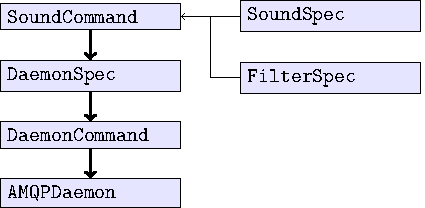
\includegraphics{figure}
  
  \caption{Dependency and compilation path hierarchy for the sound system.}
\label{fig:sshierarchy}
\end{figure}
where we have separate compilation steps to transform a \texttt{SoundCommand}
into a \texttt{DaemonSpec}, a \texttt{DaemonSpec} into a \texttt{DaemonCommand} and a
\texttt{DaemonCommand} into an \texttt{AMQPDaemon}.

These types all have different roles:
\begin{description}
\item[\tt SoundCommand] encodes all orders the system expects from
  game masters and sound designers. In order to more easily design
  datatypes, we separated out the descriptions of a sound scene and of
  a reaction trigger from the command type into the subordinate types
  \texttt{SoundSpec} and \texttt{FilterSpec}.
\item[\tt DaemonSpec] encodes, abstractly, the order types the lower
  level system accepts.
\item[\tt DaemonCommand] encodes in full detail a single order for the
  lower level system.
\item[\tt AMQPDaemon] is a datatype explicitly constructed to serialize
  through \texttt{Aeson} into a JSON package that the lower level
  system can parse.
\end{description}

Here, the \texttt{SoundCommand} type encodes all orders that the game
masters and sound designers want to be able to give to the system,
\texttt{DaemonSpec} abstractly encodes all command types the lower
level system accepts, \EZY{Missing text here?!}

All datatypes derive \texttt{Read}, \texttt{Show} and \texttt{Generic},
which allows us to automate parsing both from a Read-Evaluate-Print-Loop as well as
create automatic JSON parsers and encoders from \texttt{Aeson}. 

\subsection{SoundCommand}
\label{sec:soundspec}

Our separation of the sound scene description from the Haskell layer
control commands and the automated reactive triggers builds on their
separation into different datatypes. \EZY{What does this sentence mean?} At the top-most abstraction
level, there is a data type \texttt{SoundCommand} enumerating the
various commands that can be given to the system. 

\begin{verbatim}
data SoundCommand = 
    Define Id SoundSpec |
    Commit | 
    Restore | 
    Diagnostic |
    ReadState |
    ReadSounds | 
    Compile SoundSpec |
    ReadOut SoundSpec | 
    Execute Id SoundSpec |
    Trigger Id FilterSpec SoundCommand |
    SoundCommand :++ SoundCommand |
    Declare Id SoundCommand |
    Call Id | 
    Delete Id | 
    Nop
    deriving (Eq, Show, Read, Generic)
\end{verbatim}

There are commands for interacting with the database state storage:
\texttt{Commit} and \texttt{Restore}; commands for debugging and
analyzing what a particular sound scene description is interpreted to:
\texttt{Diagnostic}, \texttt{ReadState}, \texttt{ReadOut}; commands
for naming and recalling both sound scenes and entire commands:
\texttt{Define}, \texttt{Declare}, \texttt{Execute}, \texttt{Call},
\texttt{Delete}; and commands for triggering sound scenes either
through events by \texttt{Trigger} or through direct command by
\texttt{Execute}. Finally, there is \texttt{ReadSounds} that reports
available sound scenes up to a top level UI layer, and
\texttt{:++} for chaining commands together as well as a \texttt{Nop}
that can finish an automatically generated chain of commands for
programmatic creation of triggers and action chains. 

The definition uses the two types \texttt{SoundSpec} and
\texttt{FilterSpec} to parametrize its entries. These are given by

\begin{verbatim}
data SoundSpec = 
    Play File Segment Time Loudness |
    Loop File Segment Time Loudness |
    RadialDecay File Segment Time Loudness | 
    SoundSpec :+ SoundSpec | 
    Use Id |
    Stop Int Time |
    Fade Int Time Time Loudness |
    StopId Id Time |
    FadeId Id Time Time Loudness |
    NopS
    deriving (Eq, Show, Read, Generic)
\end{verbatim}
and
\begin{verbatim}
data FilterSpec = 
    FilterSpec :& FilterSpec |
    FilterSpec :| FilterSpec |
    MatchAll [FilterSpec] |
    MatchAny [FilterSpec] |
    MatchEvent String |
    MatchSender String |
    MatchKeyValue String String
    deriving (Eq, Show, Read, Generic, Ord)
\end{verbatim}

The sound scene specification allows for playing a sound
by name or by index, either once or on an infinite loop, and for
stopping and changing volume. These are the operations understood by
the low level system as well.

In addition to these, the Haskell layer automatically generates
packages to smoothly fade between volume settings (for a spatially
distributed decaying sound scape) and for saving and recalling sound
scenes. After an initial attempt to design the fades, we ended up building
in support for remembering the last set volume for a sound, so that
fades could be given by a target loudness rather than by start and stop
loudness settings.

The inclusion of \texttt{Nop} and \texttt{NopS} helps us automate
generation of lists of actions; together with the concatenation
constructions given by \texttt{:++} and \texttt{:+}, there is a full
monoidal structure on both these datatypes, enabling easy generation
of composite commands from lists of command parameters. 

Since the entire system actively listens to the \texttt{AMQP} traffic of the
entire game system, it was easy to include a reactive component: using
a simple regular expressions-based recognition engine, we were able
to write simple rules that would when matched trigger arbitrary
pre-constructed \texttt{SoundCommand} actions. The rules are encoded
using the type \texttt{FilterSpec} and their corresponding actions are
encoded with the \texttt{Trigger} constructor of
\texttt{SoundCommand}. All \texttt{AMQP} messages in the game system contain a
sender, an event key and some collection of key-value pairs, all of
which can be regular expression matched with the rules specified as
\texttt{FilterSpec} entities.

\subsection{DaemonSpec}
\label{sec:daemonspec}

The \texttt{DaemonSpec} type encodes the abstract payload of a single
instruction to the low-level system. An element of type
\texttt{DaemonSpec} encodes all the descriptive information needed for
a low-level system command, without containing transient information
required for emitting any particular command package. In particular,
there is a serial ID number assigned to low-level command packages to
allow later commands to modify a running sound. These ID numbers are
not added in the \texttt{DaemonSpec} representation, but rather in the
next lower representation.

\begin{verbatim}
data DaemonSpec = 
    DaemonPlay Int Segment Time Loudness |
    DaemonLoop Int Segment Time Loudness |
    DaemonStop Int Time |
    DaemonSet Int Time Loudness 
              deriving (Eq, Show)
\end{verbatim}

\subsection{DaemonCommand}
\label{sec:daemoncommand}

The \texttt{DaemonCommand} encodes a message that can be sent to the
lower-level system. In particular, the command encodes a sequential
id-number used for later modifications of looping sounds and sets up
a datatype for easy parsing for the receiving system.

\begin{verbatim}
data DaemonCommand = DaemonCommand {
      node :: Int,
      dcid :: Int,
      sound :: Int,
      time :: Int,
      volume_left :: Float,
      volume_right :: Float,
      command :: Int
    } deriving (Eq, Show, Generic)
\end{verbatim}

\subsection{AMQPDaemon}
\label{sec:amqpdaemon}

The type \texttt{AMQPDaemon} really only exists in order to wrap a
\texttt{DaemonCommand} item for serialization with \texttt{Aeson} and
transport in an \texttt{AMQP} package. The type is defined as:
\begin{verbatim}
data AMQPDaemon = AMQPDaemon {
      devent :: String,
      dsender :: String,
      dcmd :: DaemonCommand
    } deriving (Eq, Show, Generic)
\end{verbatim}
with custom JSON instances created by
\begin{verbatim}
instance FromJSON AMQPDaemon where
    parseJSON (Object v) = AMQPDaemon <$> 
                           v .: "event" <*>
                           v .: "sender" <*>
                           v .: "data"
    parseJSON _ = mzero

instance ToJSON AMQPDaemon where
    toJSON ad = object ["event" .= devent ad, 
                        "sender" .= dsender ad,
                        "data" .= dcmd ad]
\end{verbatim}

These are the only parser and encoder instances we wrote ourselves for
this project.


\subsection{Persistent state}
\label{sec:persistent-state}

There is a number of pieces of information the system needed access
to, with various levels of persistence. We designed a tiered state
type consisting of a serialisable section and a collection of
transient state properties, described by
\begin{verbatim}
data SST = SST {
      serst :: SerST,
      dbconn :: R.Connection,
      achan :: A.Channel,
      cmdid :: Int
    } 
\end{verbatim}
Here, we encode instance-specific connection data for the \texttt{Redis} database in
\texttt{dbconn}, instance-specific connection data for the \texttt{AMQP}
communication channel in \texttt{achan}, and an instance counter for
sequential command ids in \texttt{cmdid}. The rest of the state is
stored in the \texttt{serst} (\emph{ser}ializiable \emph{st}ate) field,
which is saved
to the database in order to persist settings between runs.

The serializable state in turn is given by
\begin{verbatim}
data SerST = SerST {
      soundscapes :: M.HashMap String SoundSpec,
      commands :: M.HashMap String SoundCommand,
      triggers :: [(Id,(FilterSpec, SoundCommand))],
      loops :: [(Int, (Segment, Int, Loudness))],
      tags :: M.HashMap String [Int]
    } deriving (Show, Generic)
\end{verbatim}
where we make extensive use of the strict hashmap implementation from
the \texttt{unordered-containers} package.

Here, \texttt{soundscapes} saves all named sound scape descriptions;
\texttt{commands} saves all named sound system commands;
\texttt{triggers} saves trigger definitions and is iterated through
whenever a package shows up that the system might react to;
\texttt{loops} saves currently playing loops and their most recently
known loudness; and \texttt{tags} saves a lookup table from human
readable names to command ids.

In addition to these, there is a pair of hardcoded lists defined in
the source code itself: \texttt{playable} and \texttt{loopable}.
These two lists contain the names used throughout the sound system to
refer to all playable sounds, in an order kept synchronized with
playlists on both the lower level system daemon and on the MPD
instances. From these were also derived two hashmaps \texttt{playDict} and \texttt{loopDict} to enable
faster index lookups given the names.

\subsection{Sound scape design daemon}
\label{sec:sound-scape-design}

The library described above was then used by a daemon which ran
throughout the game on one of the game control servers and reacted
dynamically to instructions arriving by \texttt{AMQP}. This daemon stored
the state in an
\texttt{IORef} and used the
callback structures in the \texttt{amqp} package to listen for and
react to \texttt{AMQP} messages. The entire logic of the server was encapsulated
in this callback and the functions it called.

The \texttt{callback} function parses out the payload of the received \texttt{AMQP}
package and checks whether it matches a regular expression. If so, it parses the contained command and acts on it; if not, it runs
the package through all defined patterns in \texttt{triggers} and runs
the associated action for each matching pattern. This linear lookup
may have been slower than more complex solutions, but it had the benefit
of being easy and reliable to design and was probably fast
enough for this application. \EZY{Well, was it fast enough?}

The function \texttt{action} executes a \texttt{SoundCommand} and
carries the entire logic of the system. This is where the data type is
translated into actual reactions. Most of the implementations are
straightforward: read the current state from the \texttt{IORef}
variable, extract relevant parts of the state, and then either assemble a package for
\texttt{AMQP} or for \texttt{Redis} and send it out, or modify the running state
according to the received instructions. By far the most involved of
these is the implementation of the \texttt{Execute} command,
responsible for sending out low-level instructions. This command constructs
\texttt{DaemonSpec} descriptions, assigns sequential command id
numbers, packs the result into \texttt{AMQP} packages, and -- depending on the
exact type of each command -- modifies the state to remember the details
of the sent commands for later recall when constructing fades or
stops.

Large swathes of the daemon code were reused to construct a command
line interface that generated \texttt{AMQP} packages for controlling the
system, allowing for an accessible debugging and programming interface.


%%% Local Variables: 
%%% mode: latex
%%% TeX-engine: default
%%% TeX-master: "tmr"
%%% End: 


\section{Usage examples}

There were different types of sounds as specified by game masters and sound designers, based on the planned usage and design requirements of the sound. There were ambient sound loops used to simulate states such as running the ships main reactor, or the sounds of massive computer banks running in the sensor processing room. There were feedback sounds triggered in response to participant actions, such as loading a torpedo or triggering a sensor sweep. These sounds mainly functioned as both confirmation to the participant that the system has registered the event and to communicate what's happening to participants in other parts of the ship. Apart from these sounds, the game masters had access to a wide variety of sounds and noises with no predetermined meaning in order to simulate everything from debris hitting the outer hull to onboard fighting, as well as pre-recorded prologues used to segue players into the game at the start of each game session.

Some sounds needed to run through an Attack-Decay-Sustain-Release sequence, with different sound files for each place, and arbitrarily long sustain-phase. Other sounds needed to trigger with fixed time intervals.

All sounds needed to be played on a set of speakers -- but not all sounds were to be played on all speakers when played. For example, sounds of airlock doors opening were played in the section containing the doors, and sections immediately adjacent to it. 

We built a setup script to handle all the sound setup in a repeatable and restartable way. The script had a \texttt{main} consisting of:
\begin{verbatim}
main = mapM_ (putStrLn . show) $ <soundlist>
\end{verbatim}
where the list of sounds was constructed in bits and pieces. We will explain and give examples for each section
of the sound list here.

We also defined, and used in most declarations for this script, a
single value for adressing all sound sites (except the engine room
sub-woofer) simultaneously
\begin{verbatim}
global = [1..11] :: [Segment] 
\end{verbatim}
as well as a utility command to help string together sound
declarations using the \texttt{SoundSpec} level concatenation
operator:
\begin{verbatim}
concatSS = foldl (:+) NopS
\end{verbatim}

\subsection{Noises and game start sounds}
\label{sec:noises}

The very easiest sounds to program for our DSL were the sounds that just needed to sound somewhere once. A single sound file to start, and let it run through.

These were all global sounds. A typical sound definition for an
environmental noise would look like the noise of a distant explosion.

\begin{listing}
\begin{verbatim}
 Trigger "explosion distant 5" 
  (MatchEvent "sound.trigger.explosion.distant.5") 
  (Execute "explo distant 5" 
   (concatSS 
    (map 
     (\i -> Play "Random/explosions/explo_distant_med_05" i 0 (100,100))
     global)))
\end{verbatim}
\caption{Reactive event definition to play the sound of a distant explosion.}
\end{listing}
This sound would be triggered by the game masters through pushing a button in their sound control console that generated a \texttt{sound.trigger.explosion.distant.5} event on the joint \texttt{AMQP} communication bus.

The same way the four different game starting sound sequences -- with mood-setting music and a spoken recap.

\begin{listing}
\begin{verbatim}
 Trigger "celestra act 3 trigger" 
  (MatchEvent "sound.trigger.act3") 
  (Execute "celestra act3" 
   (concatSS 
    (map 
     (\i -> Play "Story/Celestra_Akt3" i 0 (100,100)) 
     global)))
\end{verbatim}
\caption{Reactive event definition to start the game session starting
  sound sequences.}
\end{listing}

The same structure also took care of the game end sequences: depending on which of 6 pre-written game ending sounds was deemed appropriate a different trigger was sent over \texttt{AMQP}. This then phased over to an improvised game master epilogue spoken over the ship's PA system.

\subsection{Participant-triggered noises}
\label{sec:part-trigg-nois}

Several of the participant actions were supposed to trigger noises as well. Whenever one of the players initiated a sensor scan, or a torpedo loading procedure, sounds were triggered that corresponded to that soundscape. The only fundamental difference between these and the game-mastering sounds described above was that the triggers used were game system events. As an example, we can consider the active scanning sensor system.

\begin{listing}
\begin{verbatim}
 Trigger "dradispingtrigger" 
  (MatchEvent "space.sensor.dradis.ping") 
  (Execute "dradisping" 
   (concatSS 
    (map 
     (\i -> Play "112_active_dradis" i 1000 (80,80) :+ 
            Play "330_activating_dradis" i 0 (100,100)) 
     global))),
\end{verbatim}
\caption{The event definition for the sound system to react to a participant-triggered
  active scan ping}
\end{listing}

As a player successfully initiates an active scan, the sensor control console sends a \texttt{space.sensor.dradis.ping} message over \texttt{AMQP}. This is picked up both by the game simulation system, that reacts to the use of the active sensor in the simulation, and by the sound system that launches two sounds to be played on the entire ship. First (with time-delay 0), the sound \texttt{330\_activating\_dradis}: a synthetic voice announcing the activation of the dradis system, and then, a second later (time-delay 1000ms), the actual ping sound \texttt{112\_active\_dradis}.

\begin{figure}
  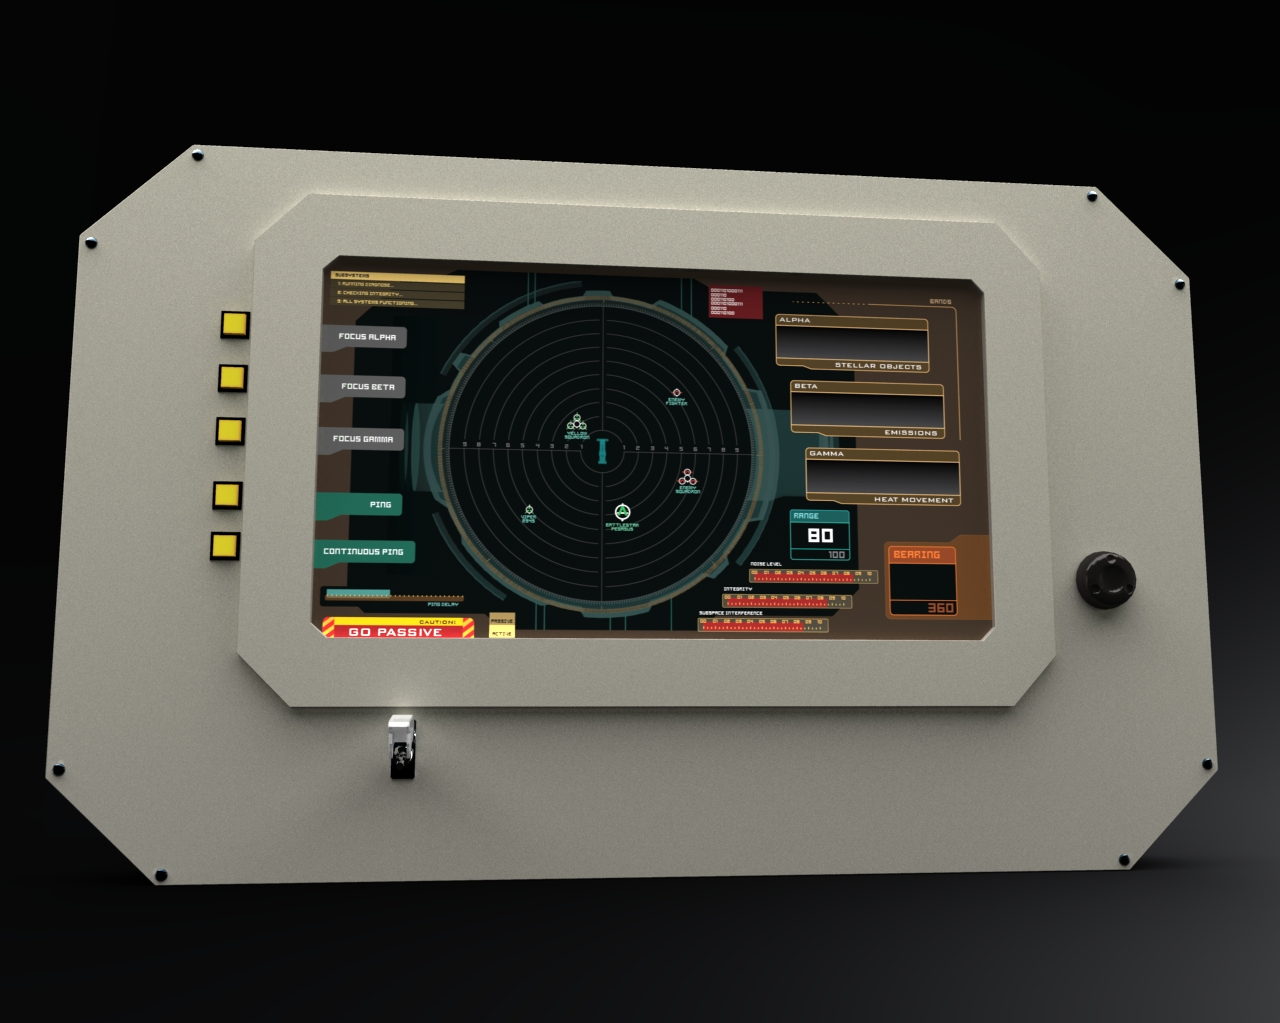
\includegraphics[width=0.4\textwidth]{img/Dradis.jpg}\hfill
  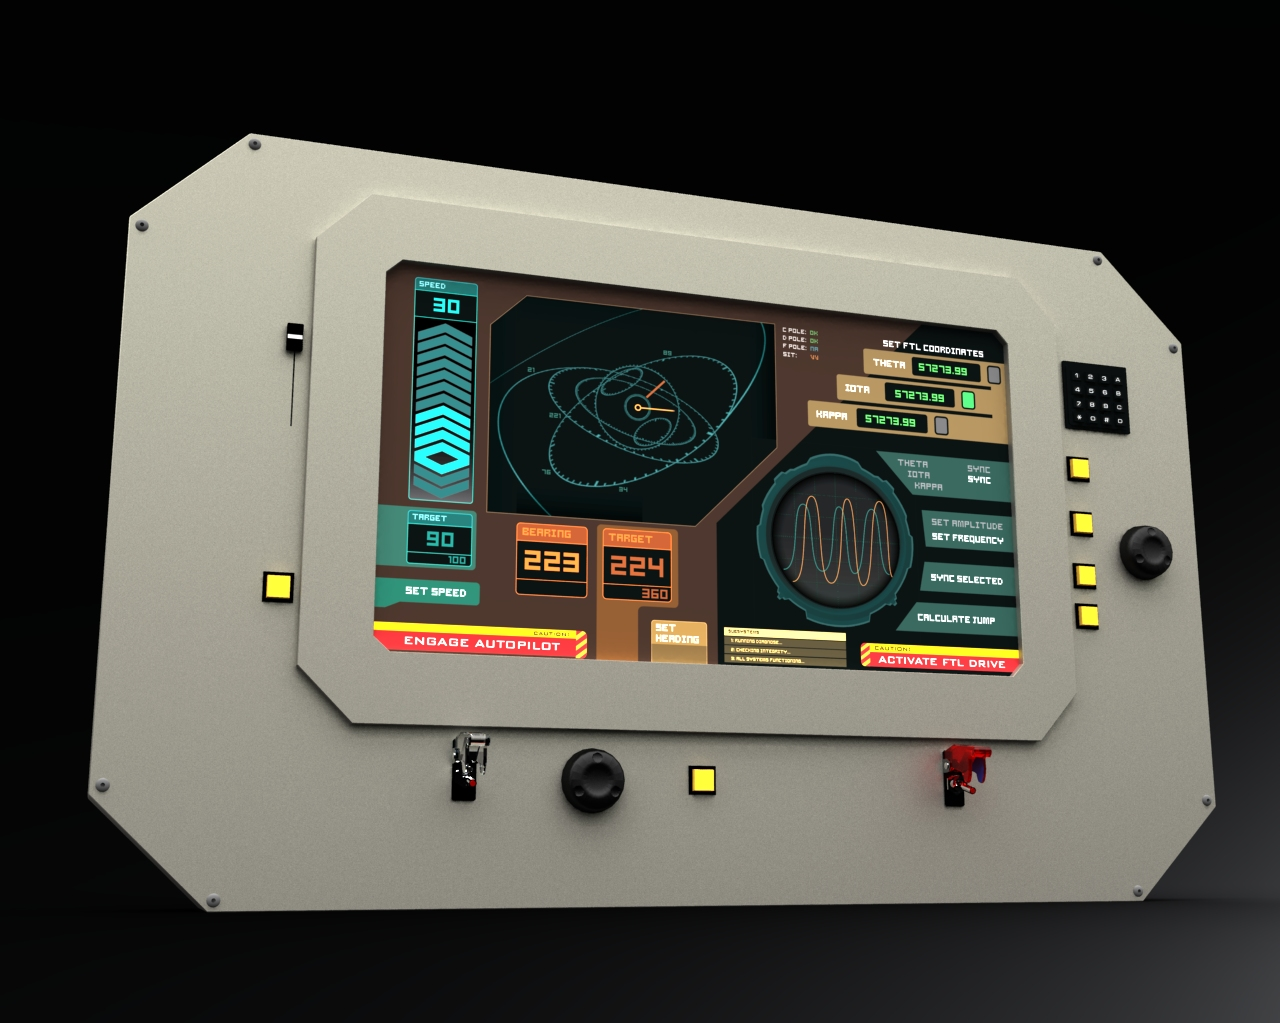
\includegraphics[width=0.4\textwidth]{img/Helm.jpg}
  \caption{The control panels for the active scanner and the FTL drive.}
  \label{fig:dradis}
\end{figure}


\subsection{Ambient loops}
\label{sec:ambient-loops}

The game was designed with three ambient noise loops: one global, with the general soundscape of a space ship in action, and two localized loops with reactor sounds and the command bridge sounds. All these needed to be started as each game session started up, and we built a single trigger to create all of them:

\begin{listing}
\begin{verbatim}
Trigger "startup loops trigger" 
 (MatchEvent "sound.trigger.startup") 
 (Execute "bridge ambience loop" 
   (concatSS 
    (map 
     (\i -> Loop "136_bridgeambience" i 0 (10,10)) 
     [8,9,10,11])) :++
  Execute "reactor ambience loop" 
   (Loop "124_reactor_run" 12 0 (60,60)) :++
  Execute "sound of celestra loop" 
   (concatSS  
    (map 
     (\i -> Loop "103_soundofcelestra" i 0 (20,20)) 
     global))),
\end{verbatim}
\caption{Reactive trigger that launches the ambient sound loops at the
start of the game.}
\end{listing}

The bridge was controlled by stations 8--11, while the large sub-woofer system for the deafening noise of the reactor engines was sound station 12. 

In addition to these loops, one more looping sound was included. If a general alarm was sounded for some reason, the blaring siren sound sat in a loop construct.

\begin{listing}
\begin{verbatim}
Trigger "alarm trigger" 
 (MatchEvent "sound.trigger.alarm") 
 (Execute "alarm" 
  (concatSS 
   (map 
    (\i -> Loop "137_generalalarm" i 0 (50,50)) 
    global))),
\end{verbatim}
\caption{Reactive trigger that launches the general alarm siren sound
  as a loop.}
\end{listing}

\subsection{Attack-decay-sustain-release}
\label{sec:attack-decay-sustain}

A large family of the sounds used in the sound scape went through a sequence of sound files, with fades between them. First, a sound that started up this particular noise sequence. Next, a loopable sound that kept things running for a while -- preferably of a length that could be determined by the game masters at will. Finally, a sound that finished the noise sequence, often indicating success or failure of the corresponding player action.

These were common enough and repetitive enough that we ended up building a specific function to generate them. In the \texttt{SoundSpec.hs} source file, we define a function \texttt{attackLoopDecay} that generates a sequence of chained sound commands.

\begin{listing}
\begin{verbatim}
attackLoopDecay :: 
  Id -> -- ^ Slug to generate ids for this command set
  Id -> -- ^ atF: attack sound
  Loudness -> -- ^ atL: attack loudness
  Int -> -- ^ t: time before fadeover
  Id -> -- ^ lpF: loop sound
  Loudness -> -- ^ lpL: loop loudness
  [Int] -> -- ^ locs: location list
  [(FilterSpec, SoundCommand)] -> -- ^ opts: Options for phasing out
  SoundCommand
attackLoopDecay slug atF atL t lpF lpL locs opts = 
 Execute (slug ++ "attack") 
         (foldl (:+) NopS (map (\i -> Play atF i 0 atL) locs)) :++
 Execute (slug ++ "loop") 
         (foldl (:+) NopS (map (\i -> Play lpF i t (0,0)) locs)) :++
 Execute (slug ++ "xfade") 
         ((FadeId (slug ++ "attack") t (t+100) (0,0)) :+
          (FadeId (slug ++ "loop") t (t+100) lpL)) :++
 (foldl (:++) Nop 
  (map 
   (\ (i,(fs,sc)) -> 
     Trigger (slug++"trigger"++(show i)) 
             fs 
             (sc :++ 
              foldl (:++) 
                    (Execute (slug++"stop") 
                             (StopId (slug ++ "loop") 0))
                    (map 
                      (\j -> Delete (slug ++ "trigger" ++ show j))
                      ([1..length opts]))
   ))
  (zip [1..] opts)))
\end{verbatim}
\caption{The \texttt{attackLoopDecay} utility function}
\end{listing}

First we execute the sound \texttt{atF} at loudness \texttt{atL} and
at all the locations in \texttt{locs}. Next, we launch the loop after
a delay of \texttt{t} and at loudness 0. We launch our cross-fade
sequence at \texttt{t+100}ms going from the attack sound to the loop
sound. Then finally we generate a family of triggers for the possible
phasing out options. Each such trigger has a numbered identifier, and
contains both the required action for the phasing out option in
\texttt{sc}, as well as commands to stop playing the loop and to clean
out all the alternative phase out options.

With this utility function in place, we are able to construct sound
sequences for potentially failing player-initiated events -- such as
using the Faster-Than-Light jump drive.

\begin{listing}
\begin{verbatim}
Trigger "ftl jump trigger" 
 (MatchEvent "space.console.ftl_jump_started") 
 ((Execute "ftl jump voice" 
   (concatSS 
    (map 
     (\i -> Play "314_initiating_FTL" i 0 (80,80)) 
     global))) :++ 
  (attackLoopDecay "ftl jump " 
     "117_FTLspinningup" (80,80) 150 
     "123_FTLspinupcomplete" (80,80) 
     global 
     [(MatchEvent "space.console.ftl_jump_completed", 
       Execute "ftl jump completed" 
        (concatSS 
         (map 
          (\i -> Play "119_FTLjump" i 0 (80,80) :+ 
                 Play "318_FTLcomplete" i 9000 (100,100)) 
          global))),
      (MatchEvent "space.console.ftl_jump_failed", 
       Execute "ftl jump failed" 
        (concatSS 
         (map 
          (\i -> Play "118_FTLfail" i 0 (80,80) :+ 
                 Play "317_FTLmalfunction" i 4000 (100,100)) 
          global)))]))
\end{verbatim}
\caption{Reactive trigger event to launch the FTL jump sound sequence,
with two options for sequence finish: one for success, one for failure.}
\end{listing}

When the FTL command console initiates a jump sequence, the
\texttt{AMQP} message \texttt{space.console.ftl\_jump\_started'} is
issued. This launches a sound system reaction that first triggers the
synthetic voice announcing ship-wide that FTL has been initiated, by
playing \texttt{314\_initiating\_FTL} everywhere.

Next, we call the \texttt{attackLoopDecay} construct to generate the
sounds for spinning up and running the FTL engine. The related sounds
are named \texttt{ftl jump attack}, \texttt{ftl jump loop},
\texttt{ftl jump xfade}, \texttt{ftl jump trigger 1}  and \texttt{ftl
  jump trigger 2}.

The two triggerable end sounds are triggered with the game master
generated \texttt{space.console.ftl\_jump\_completed} and
\texttt{space.console.ftl\_jump\_failed} messages respectively, and
play a sound and a synthetic voice message corresponding to the result.

\subsection{Countdown}
\label{sec:countdown}

Never actually used in game, we also prepared a way to generate a
synthetic voice counting down. We had pre-recorded numbers that could
be concatenated, but needed to string them together programmatically.

To do this, we adapted the game engine to send out timing signals over
\texttt{AMQP} every second, every 10 seconds, every 30 seconds and
every minute. With these, we could construct functions that generated
triggers listening to these timing signals and generating appropriate
sound commands for the countdown sequence. They were all variants of
the same fundamental structure, illustrated in Listing~\ref{lst:minutes}

\begin{listing}
\begin{verbatim}
minutes n = 
 Declare 
  ("countdown " ++ show n ++ "m0s")
  (Trigger "countdown"
   (MatchEvent "sound.heartbeat.minute")
   (Execute "countdown" 
    (concatSS 
     (map 
      (\i -> 
       Play "Countdown/T minus" i 0 (100,100) :+
       Play ("Countdown/" ++ show n) i 1000 (100,100) :+
       Play "Countdown/Minutes and counting" i 2000 (100,100)) global)) :++
    Call ("countdown " ++ show (n-1) ++ "m0s")))
\end{verbatim}
\caption{Function to parametrically define a trigger event to launch a
minute-by-minute count down sound sequence.}
\label{lst:minutes}
\end{listing}

Calling \texttt{minutes 3} would store a \texttt{SoundCommand} named
\texttt{countdown 3m0s} that generated a trigger waiting for the next
\texttt{sound.heartbeat.minute} event and then playing a synthetic
voice saying \textit{Countdown T minus three minutes and
  counting}. Finally, the event would look up and call the stored
\texttt{SoundCommand} named \texttt{countdown 2m0s}.

For the last 15 minutes, the countdown would drop down to counting
every 30 seconds; for the last minute counts every 10 seconds, for
the last 10 seconds count every second.

Access to these chains of callable commands was given to the game
masters by generating triggers through versions of the trigger given
in Listing~\ref{lst:minutetrigger}.

\begin{listing}
\begin{verbatim}
minuteTrigger n = 
 Trigger 
  ("countdown trigger " ++ show n ++ "m0s") 
  (MatchEvent ("sound.trigger.countdown." ++ show n ++ "m0s")) 
  (Call ("countdown " ++ show n ++ "m0s"))
\end{verbatim}
\caption{Game master callable triggers to launch the countdown
  sequence from a parametrizable starting time.}
\label{lst:minutetrigger}
\end{listing}

When an \texttt{AMQP} message of the form
\texttt{sound.trigger.countdown.25m0s} arrives, the trigger generated
by a call to \texttt{minuteTrigger 25} is activated. This trigger
looks up and calls the stored \texttt{SoundCommand} named
\texttt{countdown 25m0s}, which hooks into the chains of
\texttt{SoundCommand}s described above.

%%% Local Variables: 
%%% mode: latex
%%% TeX-engine: default
%%% TeX-master: "tmr"
%%% End: 


\section{Experiences}
\label{sec:experiences}

The experiences gathered in this project divide into the various
stages at which the experiences showed up. We will be dividing our
descriptions accordingly.

\subsection{Rapid development and package designs}
\label{sec:rapid-devel-pack}

It turns out that the \texttt{amqp} package expects lazy bytestrings
and the \texttt{hedis} package expects strict bytestrings. The
\texttt{bytestring} package installed had no automatic way to convert
between these -- and it took a while in the project to figure out how
to make all systems interoperate.

Several features of the resulting sound scape daemon were
direct consequences of package and platform choices. The automatically
generated serialization and parsing capabilities, both in the
\texttt{Show}/\texttt{Read} dyad and in the \texttt{Generic}
generation of JSON and bytestring serializers all mean that parsing
and serialization worked automatically and immediately. Using the
callback structure of the \texttt{amqp} library also meant that a
reactive server loop was provided essentially for free.

All these features contributed to a rapid development with large
amounts of functionality arriving early in the process.

\subsection{Interfacing to other component platforms}
\label{sec:interf-other-comp}

Since the entire project was communicating by \texttt{AMQP} with JSON-encoded
packages already, the use of these standards made interoperability
easy. One of the most difficult parts of this side of the development
process was in inspecting emitted JSON packages to figure out the
particular encoding that the \texttt{Generic}-generated JSON parser
worked with, so that appropriate and parseable structures could be
emitted from the Ruby control interfaces.

Once the reactive interfaces through the \texttt{amqp} module were in
place, it quickly became clear to us that the easiest way to provide user
interfaces to the daemon would be through a Ruby web application
front end that emitted packages crafted to trigger specific rules in
our trigger system. 

\subsection{Interfacing to creative design teams}
\label{sec:interf-creat-design}

One original expectation that did not work out as expected was to
produce a language for other users to work with; as often is the case
with large scale projects relying on voluntary work and expansive
creative vision, work on the project progressed beyond the launch of
the first performance. The sound design teams worked on sound design
far beyond the stage where they would have needed to familiarize
themselves with syntax and functionality of the sound specification
system to use it themselves.

Instead, as a compromise, we requested all relevant information to
encode the designed soundscapes; and iterated through requests for
more information and educated guesses until soundscapes were defined
and could be tested. Here, the choice of embedding the language within
Haskell paid off; the sound specification programmer was able to use
many Haskell-specific idioms and structures to produce long sequences
of parametrized and repetitive sound scape definitions. These were in
the end stored as commands stored in \texttt{triggers}, listening to specific triggering packages,
often creating new triggers for later reactions. This enabled
constructions where a player action (pressing the Load Torpedos
button) would start some sounds (a loading torpedo noise), but then
wait for game master confirmations before playing further sounds (a
loading-finished noise and a robotic voice confirmation). The later
sounds would be temporarily installed trigger definitions waiting for
a confirmation package and including cleanup code that erased all the
temporary trigger conditions after sound execution, as described in
the examples above.

\subsection{Latency in performance}
\label{sec:latency-performance}

There were latency issues in the performance use. We had, in the end,
320 trigger expressions, each carrying up to 300 sound play events in
short sequences. At the first performance, the on-site crew noticed
latencies reaching up towards 8-10 seconds between triggering action
and sound execution. Before we were able to isolate the cause of these
issues, and while we were still comparing complexity properties of the
chosen containers -- Haskell lists and strict hashmaps depending on
whether inspection of all members would be a common operation or not
-- the performance issues decreased to within a few seconds. Given the
acoustic layout of the ship, this was deemed sufficient for further
performances. 

It should be noted that the high-latency results required some
dramaturgic edits; certain sound effects were not used because they
were dependent on low latency, and thus infeasible even with the
reduced performance issues. It was decided between the first and the
second performance to run with the system as built and not try for
specific further optimizations.

\subsection{Hardware Issues}
\label{sec:hardware-issues}
An issue arouse based on the hardware. Once the system was properly deployed and the project entered
the testing and verification stage, it was discovered that before playing sounds, the system emitted a few seconds of pops and noise - regardless of the sound played. After researching the issue, this was proven to be a known issue with the RP platform, stemming from the way power supply is routed to the sound chips on the PCB. Known workarounds existed which were applied. These resolved enough of these issues for the solution to be acceptable.

\subsection{Experiences on-site}
\label{sec:experiences-on-site}

The system was installed in the war ship two days before start of the game. Installation was done in three steps; preparing clients, server-side, and on-site configuration. Since circumstances at the location were more spartan than other, off-site locations available to the team - most preparation was done in-office and then transported to the actual game location. 

Client preparation consisted of pre-loading SD cards for the Raspberry Pis with client daemons, the pre-configured sound library and connection bridges. A disk image was prepared and then duplicated onto the memory cards. This saved time at installation time, but proved to be a bad choice on-site. Certain updates could be performed over the network - but due to issues with the disk image duplication the memory cards had to be reprogrammed. This could only be done with the physical cards in hand and since the Raspberry Pis were distributed over a large area and, in many cases, in locations hard or cumbersome to reach - this proved to be a larger job than anticipated. Apart from this, pre-loading the memory cards worked very well. 

Server-side installation and configuration was done via \texttt{cabal} on the main game server. Haskell code was kept up-to-date via a Git repo and regularly synchronized from an online repository. Installation on server went as expected and was very easy to get set up. 

On-site configuration was designed to be done in three steps; physical
installation, soundscape configuration and verification. Physical
installation was cumbersome but not beyond expectations. Soundscape
configuration worked almost as expected. The \texttt{Commit} command built into the system proved invaluable since it allowed for one part of team working remotely to write an import-definition of the soundscape then send it to the on-site team who imported it into the server and then making local backups and exports.

\section{Conclusion}
\label{sec:conclusion}

Haskell as a platform, coupled with programming techniques connected
to a functional reactive programming style, to datatype construction
for domain modeling and a package collection that neatly covered all
required technological dependencies all combined to a successful
project where the sound specification system produced significant
value to the game experience and to the immersion into the game world
for the participants. Features of Haskell as a platform, and of the
packages used produced a more capable deliverable than the original
specification had expected.

We are not releasing the source code for this system openly, however
we encourage anyone interested in further details or derivative
projects to get in touch with any of the authors.


%%% Local Variables: 
%%% mode: latex
%%% TeX-engine: default
%%% TeX-master: "tmr"
%%% End: 



%\nocite{stenros2012}

%\bibliographystyle{amsalpha}
%\bibliographystyle{alpha}
\bibliography{celestra}


\end{document}

%%% Local Variables: 
%%% mode: latex
%%% TeX-engine: default
%%% TeX-master: t
%%% End: 
